\documentclass[12pt]{article}
\usepackage{a4wide}
\usepackage{NotationStyle}
\usepackage[]{algorithm2e}
%\usepackage[noend]{algorithmic}
\usepackage[english]{babel}
\usepackage{amsmath,amssymb,mathrsfs,mathtext}
\usepackage{graphics,graphicx,epsfig}
\usepackage{epstopdf}
\usepackage{fancybox,fancyhdr}
\usepackage{enumerate}
\usepackage{array}
\usepackage{color, soul}
\usepackage[normalem]{ulem}
\usepackage{arydshln}
\setlength\dashlinedash{0.2pt}
\setlength\dashlinegap{4.5pt}
\setlength\arrayrulewidth{0.2pt}

\graphicspath{ {fig/} }
\newcommand{\argmax}{\mathop{\rm arg\,max}\limits}

\begin{document}
\section{Strategies of matrix construction}
Suppose a large set of time series~$\fD=\{\bs\}$ is given. The ``object-feature'' matrix~$\bX^*$ for the multiscale autoregressive problem statement is composed of row-vectors
\[
\bs_i^\prime = [\by_i^\prime, \bx_i^\prime] = [\underbrace{s(t_i),\dots,s(t_i-\Delta t_\text{r})),}_{\by_i^\prime}
\underbrace{\dots,s(t_i-\Delta t_\text{r}-\Delta t_\text{p})}_{\bx_i^\prime}],
\]
where~$s(t)$ is an element of time series~$\bs$. Consider several strategies to decompose time series $\bs$ into segments $\Delta t_i = (t_i,\dots,t_i-\Delta t_\text{r}-\Delta t_\text{p})$ to construct  matrix $\bX^{*}$.
\begin{enumerate}
\item Row vectors $\bs_i$ cover time series without intersections. Let $\{T_{\max}, \dots, 1\}$ be the set of indices of tim series $\bs$, then thee strategy of selecting $t_i$ holds the following:
\begin{equation}\label{eq:strategy1}\{T_{\max}, \dots, 1\} = \bigsqcup_{i=1}^{M} \Delta t_i.\end{equation}
It follows from~\eqref{eq:strategy1} that $|t_{i+1} - t_i| > \dtr + \dtp$ for any $i = 1, \dots, M-1$.
\item Row vectors $\bs_i = [\y_i, \x_i]$ overlap, but target parts  $\y_i$ do not intersect:
    \begin{equation}\label{eq:strategy2}\{T_{\max}, \dots, 1\} = \bigsqcup_{i=1}{M-1} \{t_i,\dots,t_i-\Delta t_\text{r}\} \Rightarrow |t_{i+1} - t_i| > \dtr. \end{equation}
\item For each time stamp $t_i$ of the least frequent regular sampling there is correspondent row vector $\bs_i$ in $\bX^{*}$:
    \[\{T_{\max}, \dots, 1\} = \bigcup_i t_i. \]
\item Time intervals $\Delta t_i$ are selected randomly.
\item Potentially, other sensible strategies are possible.
\end{enumerate}
 Vector $\veps \in \mathbb{R}^{\dtr}$ of model residuals at time stamp $t_i$ is given by
\[\veps_i = {\y}_i - \hat{\y}_i.\]
Dependent on the way the matrix $\mathbf{X}^{*}$ is designed, there might be dependencies between components of subsequent vectors $\y_{i}$, $\y_{i+1}$.
If there are such $i, \; i' \in \cB$ that $|t_i - t_{i'}| < \dtr$, vectors $\veps_i$ and $\veps_{i'}$ overlap or contain residuals for the same time stamp. In this case define the test vector of residuals as
\[\veps(\cB) = \left\{\bar{\varepsilon}_t \left| t \in \bigcup_{i \in \cB} \{i-\dtr, \dots, i\} = \{t_{i_{\min}} - \dtr, \dots, t_{i_{\max}}\}\right.\right\}, \]
where $\bar{\varepsilon}_t$ is the average residual for the time stamp $t$.
\begin{figure}[!ht]
\centering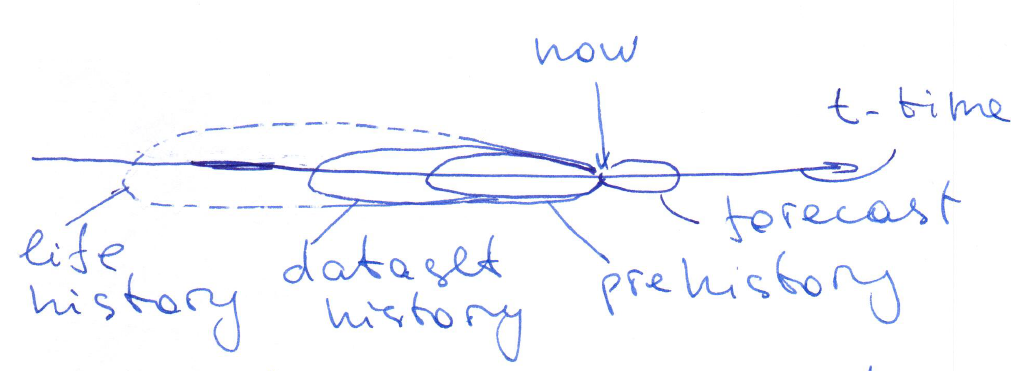
\includegraphics[width=0.8\textwidth]{online_forecasting_paradigm.png}
\label{fg:online_frc}
\caption{Online forecasting paradigm.}
\end{figure}


\begin{figure}[!ht]
\centering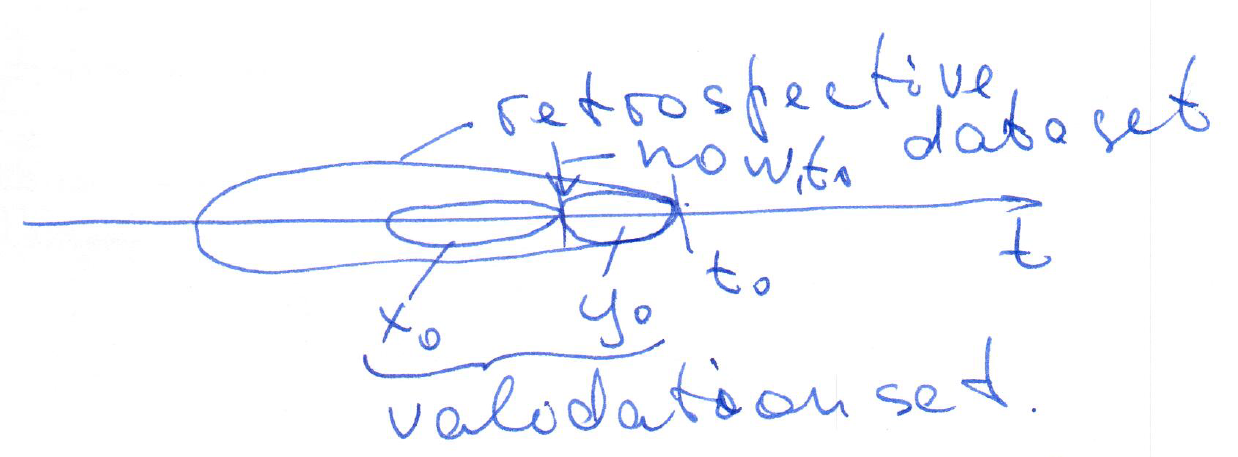
\includegraphics[width=0.8\textwidth]{retrospective_validation.png}
\label{fg:retrospective}
\caption{\hl{Retrospective forecast includes most recent samples in data set.}}
\end{figure}


\begin{figure}[!ht]
\centering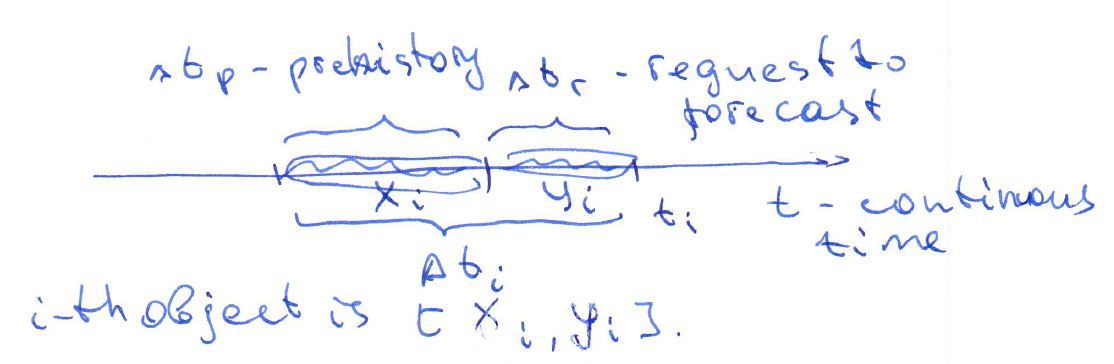
\includegraphics[width=0.8\textwidth]{draw_object.png}
\label{fg:draw}
\caption{Draw an object from time series history.}
\end{figure}
\begin{figure}[!ht]
\centering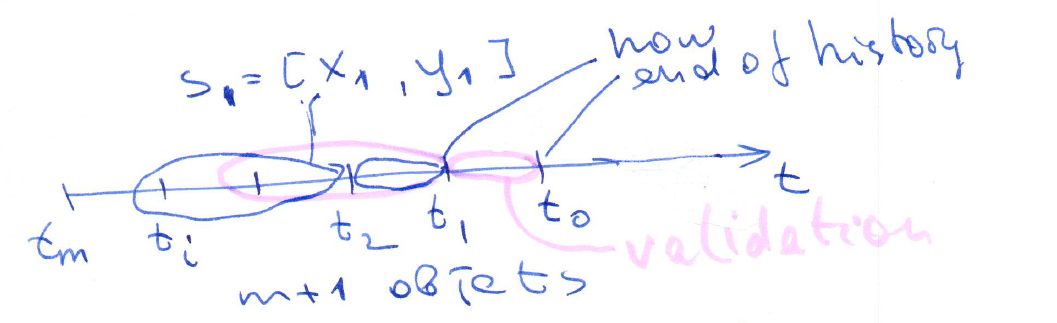
\includegraphics[width=0.8\textwidth]{design_matrix_generation.png}
\label{fg:design}
\caption{Design matrix generation.}
\end{figure}

\begin{figure}[!ht]
\centering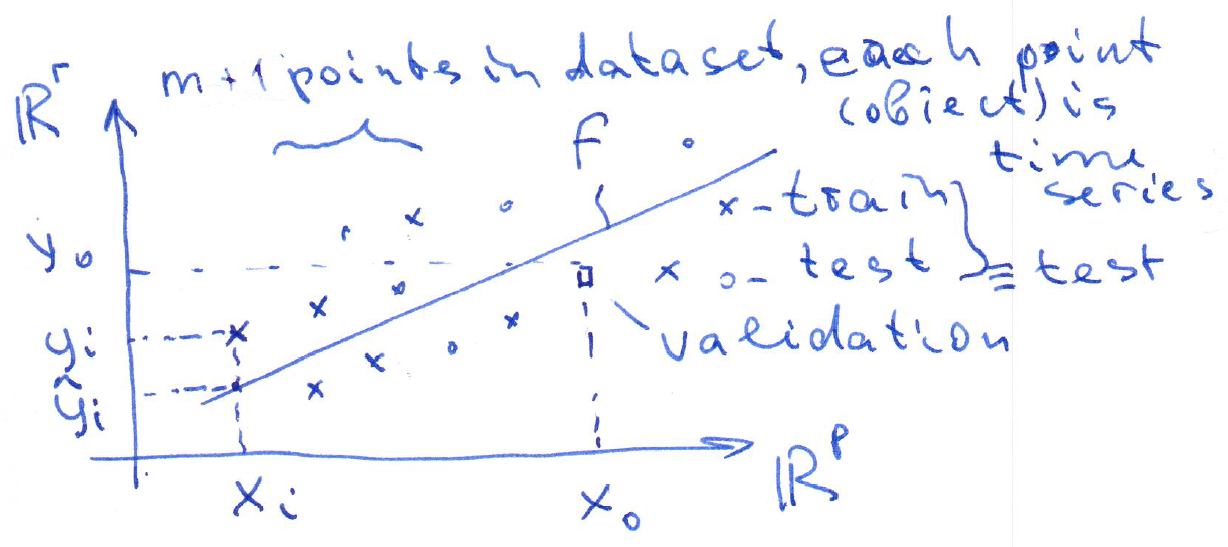
\includegraphics[width=0.8\textwidth]{forecasting_model.png}
\label{fg:forecasting}
\caption{Forecasting as regression problem.}
\end{figure}

To avoid these issues, we fix the second strategy of the $\bX$ construction.
\section{Forecast analysis}
We consider the forecast testing procedure, given by the algorithm~\ref{alg:train_test_rmse}.
Our ultimate goal is to construct a forecasting model be able to obtain forecasts at any given time $t$~\ref{fg:online}. To construct such model we have to imitate this setting, using the so-called retrospective forecast~\ref{fg:retrospective} (\hl{rolling forecasts, walking ahead predictions}). Here we conceal most recent historical samples and make predictions as if they were unknown. Then the quality of the model is evaluated according to its performance on these concealed samples. In this paper we convert the forecasting problem to regression problem,  considering the segments of time series as objects of the design matrix $\bX^{*}$~\ref{fg:draw}. Sliding~\ref{fg:design} the ``current'' time point $t$ according to the chosen strategy (1--5), we obtain the design matrix $\bX$ and further we solve the regression problem instead of forecasting problem~\ref{fg:forecasting_model}.

\begin{algorithm}[!h]
\textbf{\emph{ComputeForecastingErrors()}}

 \KwData{$\bX^{*} \in \mathbb{R}^{M\times(\dtr+\dtp)}$. Parameters: sample size $m$, train to test ratio $\alpha$.}
 \KwResult{Forecasting quality: root-mean-squared error.}
 \While{$n \leq M - m$:}{
 define, $\bX^{*}_n = [\bx^{*}_{n}, \dots, \bx^{*}_{m + n - 1}]\T$ \;
  $\bX_{\text{train}}, \; \bX_{\text{test}}, \;\bX_{\text{val}} = TrainTestSplit(\bX^{*}_n, \alpha)$\;
  train forecasting model $\fx(\x, \hat{\w}_n)$, using $\bX_{\text{train}}$ and $\bX_{\text{test}}$\;
  obtain vector of residuals $\veps = [\varepsilon_{T}, \dots, \varepsilon_{T- \dtr + 1}]$ with respect to $\bX_{\text{val}}$ \;
  compute forecasting quality:
  \[ \text{RMSE}(n)  = \sqrt{\frac{1}{\dtr} \sum_{t=0}^{\dtr} \varepsilon_{T-t}^2};\]
  $n = n + 1$ \;
  }
  Average RMSE by data splits.
  \bigskip

\textbf{\emph{TrainTestSplit()}}

\KwData{Object-feature matrix $\bX^{*} \in \mathbb{R}^{m\times(\dtr+\dtp)}$. Train to test ratio $\alpha$.}
 \KwResult{Train, test, validation matrices $\bX^{*}_{\text{train}}$, $\bX^{*}_{\text{test}}$, $\bX^{*}_{\text{val}}$.}
 Set train set and test set sizes:

 $ \quad m_{\text{train}} = \lfloor\alpha(m-1)\rfloor$ \;
 $ \quad m_{\text{test}} = m - 1 - m_{\text{train}} $ \; %(1-\alpha)(m-1)
 Decompose matrix $\bX^{*}$ into train, test, validation matrices $\bX^{*}_{\text{train}}$, $\bX^{*}_{\text{test}}$, $\bX^{*}_{\text{val}}$:
 \[\bX^{*}_{\text{train}} = \left[\begin{array}{c} \x^{*}_{\text{val}} \in \mathbb{R}^{1\times (\dtr + \dtp)}\\
 \hline
 \bX^{*}_{m_{\text{test}}} \in \mathbb{R}^{m_{\text{test}} \times (\dtr + \dtp)} \\
 \hdashline
 \bX^{*}_{m_{\text{train}}} \in \mathbb{R}^{m_{\text{train}} \times (\dtr + \dtp)}
 \end{array}\right] = \left[\begin{array}{c|c} \y_{\text{val}} & \x_{\text{val}} \\
 \hline
 \bY_{m_{\text{test}}} & \bX_{m_{\text{test}}}  \\
 \hdashline
 \bY_{m_{\text{train}}}  & \bX_{m_{\text{train}}}
 \end{array}\right]
 \]
 %$\bX^{*}_{\text{train}} = \left[\begin{array}{c|c} \y_1 & \x_1 \\ \dots &\dots, \\
% \y_{m_{\text{train}}} & \x_{m_{\text{train}}} \end{array}\right], ~~
% \bX^{*}_{\text{test}} = \left[\begin{array}{c|c} \y_1 & \x_1 \\ \dots & \dots, \\
% \y_{m_{\text{test}}}& \x_{m_{\text{test}}} \end{array}\right] $ \;
 \caption{Train-test split.}\label{alg:train_test_rmse}
\end{algorithm}

\subsection{Ensuring forecast model validity}
A valid forecast model must meet the following conditions:
\begin{itemize}
\item Mean of residuals equals to zero.
\item Residuals are stationary.
\item Residuals are not autocorrelated.
\end{itemize}
If the forecast does not meet any of these conditions, then it can be further improved by
 simply adding a constant (minus residual mean) to the model, balancing variance or including more lags. Additionally, desirable properties are normality and homoscedasticity of residuals. These properties are not necessary for an adequate model, but allow to obtain theoretical estimations of the confidence interval.

\subsection{Forecasting errors}
Hyndman~\cite{Hyndman2006} divides forecasting errors into four types:
\begin{itemize}
\item scale-dependent metrics, such as mean
absolute error
\[ MAE = \frac{1}{r}\sum_{i = 1}^{r} |\varepsilon_i|,\]
\item percentage-error metrics such as the mean absolute percent error
\[ MAPE = \frac{1}{r}\sum_{i = 1}^{r} \frac{|\varepsilon_i|}{|y_{0}(i)|}, \]
or symmetric MAPE
\[ sMAPE = \frac{1}{r}\sum_{i = 1}^{r} \frac{2|{\varepsilon}_i|}{|\hat{y}_0(i) + y_{0}(i)|}, \] \item relative-error metrics, measure
the average ratio of the errors from a designed
method to the errors $\veps^{*}$ of a benchmark method
 \[ MRAE = \frac{1}{r}\sum_{i = 1}^{r} \frac{|{\varepsilon}_i|}{{\varepsilon}^{*}_i},\]
\item and
scale-free error metrics, which express each
error as a ratio to an average error from a
baseline method:
\[ MASE = \frac{n-1}{r}\frac{\sum_{i=1}^r|\varepsilon_i|}{\sum_{j=2}^n |x_0(j) - x_0(j-1)|}. \]
\end{itemize}

\nocite{*}
\bibliographystyle{unsrt}
\bibliography{MultiscaleForecasting}


\end{document}

\paragraph{Step-by-step forecasts.}
Suppose that a forecasting model $\fx$ was built, producing forecasts
\[\hat{\y}_i = [\hat{s}(t_{i}), \dots, \hat{s}(t_{i}- \dtr)] = \fx(\x_i, \w).\]
In traditional step-by-step forecasting scheme $(k+1)$-th component of $\y_i$ depends on the forecasts of the previous $k$ components.
\[\hat{s}(t_{i}-k)  = f(\hat{\x}_i^{(k)}, \w), \quad k = 0,\dots, \dtr-1,\]
where $\hat{\x}_i^{(k)}$ includes forecasts of $k$  components of $\y_i$:
\[\hat{\x}_i^{(0)} = \x_i = [s(t_i - \dtr - 1), \dots, s(t_i - \dtr - \dtp)], \]
\[\hat{\x}^{(1)} = [\hat{s}(t_i - \dtr), s(t_i - \dtr - 1), \dots, s(t_i - \dtr - \dtp + 1)], \]
\[\dots\]
\[\hat{\x}_i^{(k)} = [\underbrace{\hat{s}(t_i - \dtr + k-1), \dots, \hat{s}(t_i - \dtr)}_{k}, s(t_i - \dtr - 1), \dots, s(t_i - \dtr - \dtp + 1)], \]
